% !TEX TS-program = pdflatex
% !TEX encoding = UTF-8 Unicode

% This is a simple template for a LaTeX document using the "article" class.
% See "book", "report", "letter" for other types of document.

\documentclass[11pt]{article} % use larger type; default would be 10pt

\usepackage[utf8]{inputenc} % set input encoding (not needed with XeLaTeX)

%%% Examples of Article customizations
% These packages are optional, depending whether you want the features they provide.
% See the LaTeX Companion or other references for full information.

%%% PAGE DIMENSIONS
\usepackage{geometry} % to change the page dimensions
\geometry{a4paper} % or letterpaper (US) or a5paper or....
\geometry{margin=1in} % for example, change the margins to 2 inches all round
% \geometry{landscape} % set up the page for landscape
%   read geometry.pdf for detailed page layout information

\usepackage{graphicx} % support the \includegraphics command and options

% \usepackage[parfill]{parskip} % Activate to begin paragraphs with an empty line rather than an indent
\usepackage{amssymb}
\usepackage{amsmath}
%%% PACKAGES
\usepackage{booktabs} % for much better looking tables
\usepackage{array} % for better arrays (eg matrices) in maths
\usepackage{paralist} % very flexible & customisable lists (eg. enumerate/itemize, etc.)
\usepackage{verbatim} % adds environment for commenting out blocks of text & for better verbatim
\usepackage{subfig} % make it possible to include more than one captioned figure/table in a single float
% These packages are all incorporated in the memoir class to one degree or another...

%%% HEADERS & FOOTERS
\usepackage{fancyhdr} % This should be set AFTER setting up the page geometry
\pagestyle{fancy} % options: empty , plain , fancy
\renewcommand{\headrulewidth}{0pt} % customise the layout...
\lhead{}\chead{}\rhead{}
\lfoot{}\cfoot{\thepage}\rfoot{}

%%% SECTION TITLE APPEARANCE
\usepackage{sectsty}
\allsectionsfont{\sffamily\mdseries\upshape} % (See the fntguide.pdf for font help)
% (This matches ConTeXt defaults)

%%% ToC (table of contents) APPEARANCE
\usepackage[nottoc,notlof,notlot]{tocbibind} % Put the bibliography in the ToC
\usepackage[titles,subfigure]{tocloft} % Alter the style of the Table of Contents
\usepackage{bbm}
\usepackage{endnotes}

\renewcommand{\cftsecfont}{\rmfamily\mdseries\upshape}
\renewcommand{\cftsecpagefont}{\rmfamily\mdseries\upshape} % No bold!
\DeclareMathOperator*{\argmax}{arg\,max}
\DeclareMathOperator*{\argmin}{arg\,min}
\usepackage{graphicx}
\graphicspath{ {./pings/} }

\newcount\colveccount
\newcommand*\colvec[1]{
        \global\colveccount#1
        \begin{pmatrix}
        \colvecnext
}
\def\colvecnext#1{
        #1
        \global\advance\colveccount-1
        \ifnum\colveccount>0
                \\
                \expandafter\colvecnext
        \else
                \end{pmatrix}
        \fi
}

\newcommand{\norm}[1]{\left\lVert#1\right\rVert}

\title{Econometrics HW2}
\author{Michael B. Nattinger\footnote{I worked on this assignment with my study group: Alex von Hafften, Andrew Smith, and Ryan Mather. I have also discussed problem(s) with Emily Case, Sarah Bass, Katherine Kwok, and Danny Edgel.}}

\begin{document}
\maketitle

\section{Question 1}
\subsection{Part i}
\begin{align*}
E[ZX'] &= E\left[\colvec{2}{Z_1}{X_2} \colvec{2}{X_1}{X_2}'\right]\\
&= \begin{pmatrix} E[Z_1X_1] &E[ Z_1X_2'] \\ E[ X_2X_1] & E[X_2 X'_2]  \end{pmatrix}\\
E[ZZ'] &= E\left[\colvec{2}{Z_1}{X_2} \colvec{2}{Z_1}{X_2}'\right]\\
&= \begin{pmatrix} E[Z_1^2] &E[ Z_1X_2'] \\ E[ X_2 Z_1] & E[X_2 X'_2]  \end{pmatrix}
\end{align*}

Note that $E[X_2X_2']$ must be invertible for either $E[ZX']$ or $E[ZZ']$ to be invertible.\footnote{$E[X_2 X_2']$ not being invertible implies the existence of some $t$ such that $E[X_2 X_2']t = 0 \Rightarrow E[(X_2't)^2] = 0 \Rightarrow E[ZX'](0,t')' = E[ZX'](0,t')' = 0$ so $E[ZX']$ and $E[ZZ']$ are not invertible.}

Block inversion implies that $E[ZX']$ is invertible iff $E[Z_1X_1] - E[Z_1X_2']E[X_2X_2']^{-1}E[X_2X_1] \neq 0$, and similarly $E[ZZ']$ is invertible iff $E[Z_1^2] - E[Z_1X_2']E[X_2X_2']^{-1}E[X_2Z_1] \neq 0$. We can rewrite these expressions as follows: $E[\hat{Z}_1 X_1] \neq 0, E[\tilde{Z}_1^2] \neq 0 $ for $\hat{Z}_1 := Z_1 - X_2'E[X_2X_2']^{-1}E[X_2Z_1].$ From FWL, for $\pi_1 = E[\tilde{Z}_1X_1].$ Together, $E[\tilde{Z}_1^2] \neq 0$ and $\pi_1 \neq 0$ imply that $E[\tilde{Z}_1X_1] \neq 0$, and the reverse direction comes from Cauchy-Schwarz:
\begin{align*}
0<E[Z_1X_1]^2 \leq E[\hat{Z}_1^2]E[ X_1^2].
\end{align*}
\subsection{Part ii}
Under homoskedasticity, $\Omega = \sigma_{U}^2E[ZX']^{-1}E[ZZ']E[XZ']^{-1}$. We again go back to block inversion and find that:
\begin{align*}
E[ZX']^{-1} &= E[\tilde{Z}_1]^{-1}\begin{pmatrix} 1 & -E[Z_1X_2']E[X_2X_2']^{-1} \\ \dots & \dots \end{pmatrix},
\end{align*}
where the second block row does not enter into the upper left entry of $\Omega$. We then have the following:
\begin{align*}
\Omega_{1,1} &= \frac{ \sigma_{U}^2}{E[Z_1X_1']^2} (E[Z_1]^2 - E[Z_1X_2']^{-1}E[X_2Z_1])\\
&= \frac{\sigma_{U}^2E[\tilde{Z}^2_1]}{E[Z_1X_1']^2}\\
&= \frac{\sigma_{U}^2]}{E[\tilde{Z}_1^2]\pi_1^2}
\end{align*}
\subsection{Part iii}
$\pi$ is the population projection (regression) coefficients mapping $Z$ into $X_1$, and $\tilde{Z}$ is $Z$ residualized at the population level with respect to $X_2$.
\subsection{Part iv}
\begin{align*}
E[\tilde{Z}_1X_2] =  E[X_2Z_1 - X_2X_2'E[X_2X_2']^{-1}E[X_2Z_1]] = 0.
\end{align*}

The above expression implies the following:
\begin{align*}
E[\tilde{Z}_1X_2E[X_2X_2']^{-1}E[X_2E[X_1|Z]]] &= 0\\
E[\tilde{Z}_1X_1] = E[\tilde{Z}_1E[X_1|Z]] - E[\tilde{Z}_1X_2E[X_2X_2']^{-1}E[X_2E[X_1|Z]]] &= E[\tilde{Z}Z_{*}]\\ 
\end{align*}
We apply Cauchy-Schwarz to achieve the desired inequality:
\begin{align*}
\Omega_{1,1} &= \frac{\sigma^2_UE[\tilde{Z}^2_1]}{E[\tilde{Z}Z_{*}]^2} \\
&\geq \frac{\sigma^2_UE[\tilde{Z}^2_1]}{E[\tilde{Z}^2]E[Z_{*}^2]}\\
&=    \frac{\sigma^2_U}{E[Z_{*}^2]}
\end{align*}

We will achieve the lower bound when $Z_{*} = \tilde{Z}_1\pi_1$. This occurs when $E[X_1|Z] = Z_1\pi_1 + X_2'\pi_2$.
\subsection{Part v}
If $X_2$ is just a constant, $\tilde{Z} = Z-E[Z],E[\tilde{Z}_{1}^2] = Var(Z_1), E[\tilde{Z}_1X_1] = Cov(Z_1,X_1).$ Thus,

\begin{align*}
\Omega_{1,1} &= \frac{\sigma_U^2Var(Z_1)}{Cov(Z_1,X_1)^2}.
\end{align*}

\section{Question 2}
\subsection{Part i}
\begin{align*}
E[h(Z)(Y-X\beta)] &= E[h(Z)(X(\beta_1 - \beta)) + U)]\\
&= E[h(Z)X](\beta_1 - \beta) + E[h(Z)U].
\end{align*}
If exogeneity holds, $E[h(Z)U] = E[h(Z)E[U|Z]] = 0$ so $E[h(Z)(Y-X\beta)] = 0 \iff \beta_1 = \beta.$
\subsection{Part ii}
Define $\hat{\beta}^{h}_1$ as the solution to the following:
\begin{align}
\frac{1}{n}\sum_{i}(h(Z_i)(Y_i - X_i \hat{\beta}^{h}_1)) = 0\\
\Rightarrow \frac{1}{n}\sum_{i}(h(Z_i)(Y_i)) - \frac{1}{n}\sum_{i}(h(Z_i)X_i) \hat{\beta}^{h}_1 &= 0\\
\Rightarrow \hat{\beta}^{h}_1 &= \left[\frac{1}{n}\sum_{i}(h(Z_i)X_i)\right]^{-1}\frac{1}{n}\sum_{i}(h(Z_i)(Y_i))
\end{align}
\subsection{Part iii}
By applying the law of large numbers twice and continuous mapping theorem, we reach the following probability limit:
\begin{align*}
\hat{\beta}^{h}_1 &\rightarrow_p [E[h(Z)X]]^{-1}E[h(Z)Y]\\
&= [E[h(Z)X]]^{-1}E[h(Z)(X\beta_1 +U)]\\
&= [E[h(Z)X]]^{-1}E[h(Z)X]\beta_1 + [E[h(Z)X]]^{-1}E[h(Z)U]\\
&=\beta_1 + [E[h(Z)X]]^{-1}E[h(Z)E[U|Z]]\\
&= \beta_1.
\end{align*}

Now, we have the following:
\begin{align*}
\sqrt{n}(\hat{\beta}^h_1 - \beta_1) &=  \left[\frac{1}{n}\sum_{i}(h(Z_i)X_i)\right]^{-1}\frac{1}{\sqrt{n}}\sum_{i}(h(Z_i)(U_i))
\end{align*}
By LLN, $\frac{1}{n}\sum_{i}(h(Z_i)X_i)\rightarrow_p E[h(Z)X].$ Also, by the CLT,
\begin{align*}
\frac{1}{\sqrt{n}}\sum_{i}(h(Z_i)(U_i)) \rightarrow_d N(0,V)
\end{align*}
where $V = Var(h(Z)U) = E[(h(Z))^2 U^2] - E[h(Z)U]^2 = E[(h(Z))^2 U^2] - E[h(Z)E[U|Z]]^2 = E[(h(Z))^2 U^2].$ By the continuous mapping theorem,
\begin{align*}
\sqrt{n}(\hat{\beta}^h_1 - \beta_1) &\rightarrow_d N(0,E[h(Z)X]^{-2}E[(h(Z))^2U^2] )
\end{align*}

\subsection{Part iv}
We have from part (iii) that $\Omega^h = E[h(Z)X]^{-2}E[(h(Z))^2U^2]$. By applying the law of iterated expectations and then Cauchy-Schwarz,
\begin{align*}
\Omega^h &= \frac{E[(h(Z))^2U^2]}{E[h(Z)X]^2}\\
&=  \frac{E[(h(Z))^2E[U^2|Z]]}{E\left[[h(Z)\sqrt{E[U^2|Z]}\frac{E[X|Z]}{\sqrt{E[U^2|Z]}}\right]^2}\\
&\geq   \frac{E[(h(Z))^2E[U^2|Z]]}{E\left[(h(Z))^2E[U^2|Z]\right]\left(\frac{E[X|Z]^2}{E[U^2|Z]}\right)}\\
&= \left(\frac{E[X|Z]^2}{E[U^2|Z]}\right)^{-1}
\end{align*}

We can find $h_{*}$ which achieves this lower bound. Let $h_{*} = E[X|Z](E[U^2|Z])^{-1}.$ Then,
\begin{align*}
\Omega^{h_{*}} &= \frac{E[(h_{*}(Z))^2U^2]}{E[h_{*}(Z)X]^2}\\
&=  \frac{E[(E[X|Z](E[U^2|Z])^{-1})^2E[U^2|Z]]}{E[E[X|Z](E[U^2|Z])^{-1}E[X|Z]]^2} \\
&= \frac{E[E[X|Z]^2(E[U^2|Z])^{-1}]}{E[E[X|Z]^2(E[U^2|Z])^{-1}]^2}\\
&= \left(\frac{E[X|Z]^2}{E[U^2|Z]}\right)^{-1}.
\end{align*}
\section{Question 3}
\begin{center}
\begin{tabular}{ll}
& Results \\ 
\hline 
Beta hat & 0.10842 \\ 
SE & 0.01948 \\ 
\hline 
\end{tabular}
\end{center}

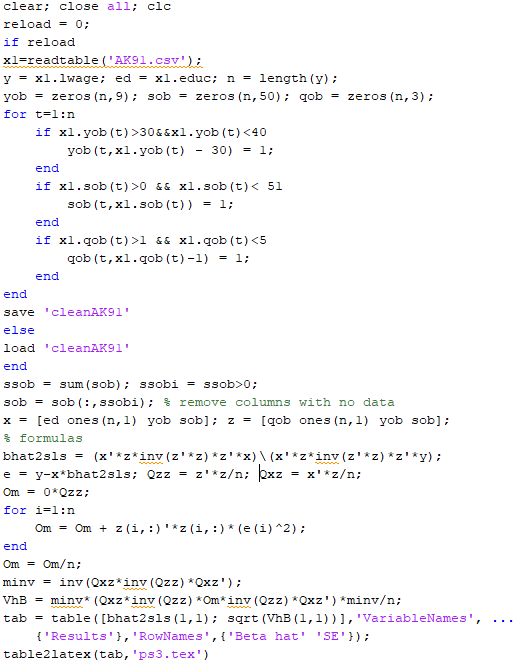
\includegraphics{hw3q3}
\end{document}
